% !TEX TS-program = xelatex
\documentclass[10pt,landscape,a4paper]{article}
%\usepackage[utf8]{inputenc}
%\usepackage[ngerman]{babel}
\usepackage{tikz}
\usetikzlibrary{shapes,positioning,arrows,fit,calc,graphs,graphs.standard}
\usepackage[nosf]{kpfonts}
\usepackage[t1]{sourcesanspro}
%\usepackage[lf]{MyriadPro}
%\usepackage[lf,minionint]{MinionPro}
\usepackage{multicol}
\usepackage{wrapfig}
\usepackage[top=0mm,bottom=1mm,left=0mm,right=1mm]{geometry}
\usepackage[framemethod=tikz]{mdframed}
\usepackage{microtype}
\usepackage{lastpage}
%\usepackage{physics}
\usepackage{datetime}
\yyyymmdddate
\renewcommand{\dateseparator}{-}
\let\bar\overline

\definecolor{myblue}{cmyk}{1,.72,0,.38}

\def\firstcircle{(0,0) circle (1.5cm)}
\def\secondcircle{(0:2cm) circle (1.5cm)}

\colorlet{circle edge}{myblue}
\colorlet{circle area}{myblue!5}

\tikzset{filled/.style={fill=circle area, draw=circle edge, thick},
    outline/.style={draw=circle edge, thick}}

\pgfdeclarelayer{background}
\pgfsetlayers{background,main}

\everymath\expandafter{\the\everymath \color{myblue}}
%\everydisplay\expandafter{\the\everydisplay \color{myblue}}


\renewcommand{\baselinestretch}{.8}
\pagestyle{empty}

\global\mdfdefinestyle{header}{%
linecolor=gray,linewidth=1pt,%
leftmargin=0mm,rightmargin=0mm,skipbelow=0mm,skipabove=0mm,
}

\newcommand{\header}{
\begin{mdframed}[style=header]
\footnotesize
\sffamily
MA1521 Finals Cheatsheet v1.2 (\today)\\
by~Julius~Putra~Tanu~Setiaji,~page~\thepage~of~\pageref{LastPage}
\end{mdframed}
}
%\usepackage{chngcntr}

\usepackage{pgfplots}
\pgfplotsset{compat=1.8}
\counterwithin*{equation}{section}
\counterwithin*{equation}{subsection}
\usepackage{enumitem}
\newlist{legal}{enumerate}{10}
\setlist[legal]{label*=\arabic*.,leftmargin=4mm}
\setlist[itemize]{leftmargin=4mm}
\setlist{itemsep=0mm,topsep=1mm,leftmargin=4mm}
\newenvironment{descitemize} % a mixture of description and itemize
{\begin{description}[leftmargin=*,before=\let\makelabel\descitemlabel]}
{\end{description}}

\newcommand{\descitemlabel}[1]{%
\textbullet\ \textbf{#1}%
}
\makeatletter



\renewcommand{\section}{\@startsection{section}{1}{0mm}%
                                {.2ex}%
                                {.2ex}%x
                                {\color{myblue}\sffamily\small\bfseries}}
\renewcommand{\subsection}{\@startsection{subsection}{1}{0mm}%
                                {.2ex}%
                                {.2ex}%x
                                {\sffamily\bfseries}}



\def\multi@column@out{%
   \ifnum\outputpenalty <-\@M
   \speci@ls \else
   \ifvoid\colbreak@box\else
     \mult@info\@ne{Re-adding forced
               break(s) for splitting}%
     \setbox\@cclv\vbox{%
        \unvbox\colbreak@box
        \penalty-\@Mv\unvbox\@cclv}%
   \fi
   \splittopskip\topskip
   \splitmaxdepth\maxdepth
   \dimen@\@colroom
   \divide\skip\footins\col@number
   \ifvoid\footins \else
      \leave@mult@footins
   \fi
   \let\ifshr@kingsaved\ifshr@king
   \ifvbox \@kludgeins
     \advance \dimen@ -\ht\@kludgeins
     \ifdim \wd\@kludgeins>\z@
        \shr@nkingtrue
     \fi
   \fi
   \process@cols\mult@gfirstbox{%
%%%%% START CHANGE
\ifnum\count@=\numexpr\mult@rightbox+2\relax
          \setbox\count@\vsplit\@cclv to \dimexpr \dimen@-1cm\relax
\setbox\count@\vbox to \dimen@{\vbox to 1cm{\header}\unvbox\count@\vss}%
\else
      \setbox\count@\vsplit\@cclv to \dimen@
\fi
%%%%% END CHANGE
            \set@keptmarks
            \setbox\count@
                 \vbox to\dimen@
                  {\unvbox\count@
                   \remove@discardable@items
                   \ifshr@nking\vfill\fi}%
           }%
   \setbox\mult@rightbox
       \vsplit\@cclv to\dimen@
   \set@keptmarks
   \setbox\mult@rightbox\vbox to\dimen@
          {\unvbox\mult@rightbox
           \remove@discardable@items
           \ifshr@nking\vfill\fi}%
   \let\ifshr@king\ifshr@kingsaved
   \ifvoid\@cclv \else
       \unvbox\@cclv
       \ifnum\outputpenalty=\@M
       \else
          \penalty\outputpenalty
       \fi
       \ifvoid\footins\else
         \PackageWarning{multicol}%
          {I moved some lines to
           the next page.\MessageBreak
           Footnotes on page
           \thepage\space might be wrong}%
       \fi
       \ifnum \c@tracingmulticols>\thr@@
                    \hrule\allowbreak \fi
   \fi
   \ifx\@empty\kept@firstmark
      \let\firstmark\kept@topmark
      \let\botmark\kept@topmark
   \else
      \let\firstmark\kept@firstmark
      \let\botmark\kept@botmark
   \fi
   \let\topmark\kept@topmark
   \mult@info\tw@
        {Use kept top mark:\MessageBreak
          \meaning\kept@topmark
         \MessageBreak
         Use kept first mark:\MessageBreak
          \meaning\kept@firstmark
        \MessageBreak
         Use kept bot mark:\MessageBreak
          \meaning\kept@botmark
        \MessageBreak
         Produce first mark:\MessageBreak
          \meaning\firstmark
        \MessageBreak
        Produce bot mark:\MessageBreak
          \meaning\botmark
         \@gobbletwo}%
   \setbox\@cclv\vbox{\unvbox\partial@page
                      \page@sofar}%
   \@makecol\@outputpage
     \global\let\kept@topmark\botmark
     \global\let\kept@firstmark\@empty
     \global\let\kept@botmark\@empty
     \mult@info\tw@
        {(Re)Init top mark:\MessageBreak
         \meaning\kept@topmark
         \@gobbletwo}%
   \global\@colroom\@colht
   \global \@mparbottom \z@
   \process@deferreds
   \@whilesw\if@fcolmade\fi{\@outputpage
      \global\@colroom\@colht
      \process@deferreds}%
   \mult@info\@ne
     {Colroom:\MessageBreak
      \the\@colht\space
              after float space removed
              = \the\@colroom \@gobble}%
    \set@mult@vsize \global
  \fi}

\makeatother
\setlength{\parindent}{0pt}
\setlength\columnsep{1.5pt}
\setlength\columnseprule{0.1pt}
\begin{document}

\footnotesize
\begin{multicols*}{4}
  \raggedcolumns
  \section{Trigo Formulae}
  \begin{descitemize}
    \item $\sin^2 \theta + \cos^2 \theta = 1$, $\sin 2\theta = 2\sin \theta \cos \theta$
    \item $\sin(A \pm B) = \sin A\cos B \pm \sin B \cos A$
    \item $\cos(A \pm B) = \cos A \cos B \mp \sin A \sin B$
    \item $\tan(A \pm B) = \frac{\tan A \pm \tan B}{1 \mp \tan A \tan B}$, $\tan 2\theta = \frac{2\tan \theta}{1-\tan^2 \theta}$
    \item $\cos 2\theta = cos^2 \theta - sin^2 \theta = 2\cos ^2 \theta - 1 = 1 - 2\sin^2 \theta$
    \item $\sin P + \sin Q = 2\sin \frac{1}{2}(P+Q) \cos \frac{1}{2}(P-Q)$
    \item $\sin P - \sin Q = 2\cos \frac{1}{2}(P+Q) \sin\frac{1}{2}(P-Q)$
    \item $\cos P + \cos Q = 2\cos \frac{1}{2}(P+Q) \cos\frac{1}{2}(P-Q)$
    \item $\cos P - \cos Q = -2\sin \frac{1}{2}(P+Q) \sin\frac{1}{2}(P-Q)$
    \item $a^2 = b^2+c^2-2bc\cos\theta$ and $\frac{a}{\sin a} = \frac{b}{\sin b}$
  \end{descitemize}
  \section{Functions and Limits}
  \subsection*{Existence of Limits}
  $\lim\limits_{x\to a} f(x)$ only exists when:
  \begin{descitemize}
    \item $\lim\limits_{x\to a^-} f(x) = \lim\limits_{x\to a^+} f(x)$ (limit from left = right)
    \item For $a=\infty$ or $-\infty$, only if $f(x)$ \textbf{does not} oscillate
  \end{descitemize}
  \subsection*{Rules of Limits}
  \begin{enumerate}
    \item $\lim\limits_{x\to a} (f \pm g)(x) = \lim\limits_{x\to a}f(x) \pm \lim\limits_{x\to a} g(x)$
    \item $\lim\limits_{x\to a} f(x)g(x) = \lim\limits_{x\to a}f(x) \lim\limits_{x\to a}g(x)$
    \item $\lim\limits_{x\to a} \frac{f(x)}{g(x)} = \frac{\lim\limits_{x\to a} f(x)}{\lim\limits_{x\to a} g(x)}$ provided $\lim\limits_{x\to a} g(x) \neq 0$
    \item $\lim\limits_{x\to a} kf(x) = k \lim\limits_{x\to a} f(x)$
  \end{enumerate}
  \subsection*{Continuity}
  $f$ is continuous at point $a \Leftrightarrow \lim\limits_{x\to a} f(x) = f(a)$
  \subsection*{L'H\^opital's Rule}
  Suppose:
  \begin{enumerate}
    \item $f$ and $g$ are differentiable
    \item $f(a)=g(a)=0$
    \item $g'(x)\neq0$ for all $x \in I \setminus {a}$
  \end{enumerate}
  Then $\lim\limits_{x\to a}\frac{f(x)}{g(x)} = \lim\limits_{x\to a}\frac{f'(x)}{g'(x)}$\\
  \begin{descitemize}
    \item Use L'H\^opital's Rule for $\frac{0}{0}$ and $\frac{\infty}{\infty}$ forms.

    \item Common: $\lim\limits_{x\to\frac{\pi^-}{2}}(\sin x)^{\tan x} = \lim\limits_{x\to\frac{\pi^-}{2}} e^{\ln(\sin x)^{\tan x}}\\=e^{\lim\limits_{x\to\frac{\pi^-}{2}}\tan x\ln(\sin x)}=e^{\lim\limits_{x\to\frac{\pi^-}{2}}\frac{\ln(\sin x)}{\cot x}}$ (now in $\frac{0}{0}$ form)
    \item Tips:
    \begin{enumerate}
      \item Convert $0 \cdot \infty, \infty - \infty$ by algebra manip
      \item Convert $ 1^\infty, \infty^0, 0^0$ by first taking $\ln$
    \end{enumerate}
  \end{descitemize}

  \section{Derivative}
  The derivative of $f$ at point $a$ is $\lim\limits_{x\to a} \frac{f(x) - f(a)}{x - a}$, \\ denoted by $f'(a)$ provided the limit exists.\\
  $f'(a)=\lim\limits_{x\to a} \frac{f(x) - f(a)}{x - a}=\lim\limits_{h\to0}\frac{f(a+h) - f(a)}{h}=\left.\frac{dy}{dx}\right\rvert_{x=a}$\\
  $f'(a)=$ slope of tangent at pt $a$
  \subsection*{Some properties}
  \begin{descitemize}
    \item $f'(a)$ exists $\Rightarrow f(x)$ is smooth ($\therefore$ continuous) at $a$
    \item $f'(a)$ does not exist at \textbf{discontinuity, corner,} and \textbf{vertical tangent.}
  \end{descitemize}
  Since derivative is limit, if lim from left $\neq$ right, then $f'(a)$ does not exist.
  \subsection*{Formulae}
  \begin{tabular}{c | c}
    \hline
    Function    & Derivative                  \\ \hline
    $(f(x))^n$  & $nf'(x)f(x)^{n-1}$          \\ \hline
    $\sin f(x)$ & $f'(x)\cos f(x)$            \\ \hline
    $\cos f(x)$ & $-f'(x)\sin f(x)$           \\  \hline
    $\tan f(x)$ & $f'(x)\sec^2 f(x)$          \\ \hline
    $\cot f(x)$ & $-f'(x)\csc^2 f(x)$         \\ \hline
    $\sec f(x)$ & $f'(x)\sec f(x) \tan f(x)$  \\ \hline
    $\csc f(x)$ & $-f'(x)\csc f(x) \cot f(x)$ \\ \hline
    $a^f(x)$    & $f'(x)a^{f(x)} \ln a$       \\ \hline
  \end{tabular}\\
  \begin{tabular}{c | c}
    \hline
    Function     & Derivative                 \\ \hline
    $k$          & $0$                        \\ \hline
    $e^f(x)$     & $f'(x)e^{f(x)}$            \\ \hline
    $\log_af(x)$ & $\frac{f'(x)}{f(x) \ln a}$ \\ \hline
    $\ln f(x)$   & $\frac{f'(x)}{f(x)}$       \\ \hline
  \end{tabular}
  \begin{tabular}{c | c}
    \hline
    Function        & Derivative                       \\ \hline
    $\sin^{-1}f(x)$ & $\frac{f'(x)}{\sqrt{1-f(x)^2}}$  \\ \hline
    $\cos^{-1}f(x)$ & $-\frac{f'(x)}{\sqrt{1-f(x)^2}}$ \\ \hline
    $\tan^{-1}f(x)$ & $\frac{f'(x)}{1+f(x)^2}$         \\ \hline
  \end{tabular}
  \subsection*{Rules of Differentiation}
  \begin{descitemize}
    \item $(kf)'(x) = kf'(x)$
    \item $(f \pm g)'(x) = f'(x) \pm g'(x)$
    \item $\frac{d}{dx}uv=u\frac{dv}{dx}+v\frac{du}{dx}$
    \item $\left(\frac{f}{g}\right)'(x) = \frac{f'(x)g(x)-f(x)g'(x)}{(g(x))^2}$
    \item $\frac{d}{dx} f(g(x))=f'(g(x)) g'(x)$ or  $\frac{dy}{dx}=\frac{dy}{du}\cdot\frac{du}{dx}$
  \end{descitemize}
  \subsection*{Parametric Differentiation}
  Given $\begin{cases}
      y=u(t) \\
      x=v(t)
    \end{cases}$
  , we have $\frac{dy}{dx}=\frac{\frac{dy}{dt}}{\frac{dx}{dt}}$
  \begin{descitemize}
    \item [Second derivative] \leavevmode \\
    $\frac{d^2y}{dx^2} = \frac{d}{dx}\left(\frac{dy}{dx}\right)$ then do implicit differentiation w.r.t $x$
    \item [Polar equation] ($r=a\theta$): $x=r\cos\theta, y=r\sin\theta$
  \end{descitemize}
  \subsection*{Implicit Differentiation}
  Differentiate w.r.t. to var, then multiply by $\frac{d\text{<var>}}{dx}$
  Common: $y=x^x \iff \ln y = x \ln x$
  \subsection*{Higher Order Derivatives}
  The $n$-th derivative is denoted by $\frac{d^ny}{dx^n}$ or $f^{(n)}(x)$
  \subsection*{Maxima and Minima}
  \begin{descitemize}
    \item [$f(c)$ is Local Maximum] if $f(c) \geq f(x)$ for $x$ near $c$
    \item [$f(c)$ is Local Minimum] if $f(c) \leq f(x)$ for $x$ near $c$
    \item [$f(c)$ is abs maximum] if $f(c) \geq f(x) \forall x \in$ domain
    \item [$f(c)$ is abs minimum] if $f(c) \leq f(x) \forall x \in$ domain
    \item [Critical Point]:\\
    Let $f$ be a function with domain $D$. An interior point (not end-point) $c$ in $D$ is called a \textbf{Critical Point} of $f$ if $f'(c)=0$ of $f'(c)$ does not exist.
    \item [Method to find extreme values of $f$]: \\
    Check critical points of $f$, end-points of domain $D$
  \end{descitemize}
  \subsection*{Method to Find Local Extreme values}
  A function may not have a local extreme at a critical pt. Check using 1st/2nd derivative tests.
  \begin{descitemize}
    \item [1st Derivative Test]: \\
    Assume $c \in (a,b)$ is a critical point of $f$
    \begin{enumerate}
      \item $f'(x)>0$ for $x \in (a,c)$ and $f'(x)<0$ for $x \in (c,b)$, then $f$ is a \textbf{local maximum}
      \item $f'(x)<0$ for $x \in (a,c)$ and $f'(x)>0$ for $x \in (c,b)$, then $f$ is a \textbf{local minimum}
    \end{enumerate}
    \item [2nd Derivative Test]: \\
    $f'(c) = 0$ $\begin{cases}
        f''(c)<0 \iff f \text{ has local max at } c \\
        f''(c)>0 \iff f \text{ has local min at } c
      \end{cases}$\\
    Note: if $f'(c)=0$ and $f''(c)=0$ then 2nd derivative test fails. Use 1st derivative test.
  \end{descitemize}
  \subsection*{Method to Find Absolute Extreme Values}
  \begin{enumerate}
    \item Find all critical points $c$ in the interior
    \item Evaluate $f(c)$, where $c$ is a critical or end point
    \item The largest and smallest of these values will be abs max \& min respectively
  \end{enumerate}
  \subsection*{Increasing and Decreasing Functions}
  Test for Monotonic Functions ($f:I$ (interval) $\rightarrow \mathbb{R}$):

  \begin{descitemize}
    \item $f'(x)>0$ for any $x$ in $I \Rightarrow f$ is \textbf{increasing} on $I$
    \item $f'(x)<0$ for any $x$ in $I \Rightarrow f$ is \textbf{decreasing} on $I$
  \end{descitemize}
  \subsection*{Concativity}
  $\begin{cases}
      f''(x)<0 \Leftrightarrow f'(x)\text{ is decreasing} \Leftrightarrow \text{Concave Down} \\
      f''(x)>0 \Leftrightarrow f'(x)\text{ is increasing} \Leftrightarrow \text{Concave Up}
    \end{cases}$
  \subsection*{Points of Inflection}
  Let $f:I \rightarrow \mathbb{Z}$ and $c \in I$.\\
  $c$ is a pt of inflection of $f$ if $f$ is continuous at $c$ and the concavity of $f$ changes at $c$.\\
  In another word: c is pt of inflection $\rightarrow f''(c)=0$ (but not the reverse -- c is a pt of inflection only if $f''(c)$ crosses from (+) to (-) and vice versa.)

  \section{Integration}
  \subsection*{Indefinite Integral}
  Denoted by $\int f(x)dx = F(x) + C$
  \subsection*{Geometrical Interpretation}
  All curves $y=F(x) + C$ s.t. their slopes at $x$ are $f(x)$
  \subsection*{Rules of Indefinite Integration}
  \begin{enumerate}
    \item $\int kf(x)dx=k\int f(x)dx$
    \item $\int -f(x)dx=-\int f(x)dx$
    \item $\int [f(x) \pm g(x)] dx=\int f(x)dx \pm \int g(x)dx$
  \end{enumerate}
  \subsection*{Integral Formulae}
  \begin{tabular}{c|c}
    \hline
    \textbf{Function}     & \textbf{Integral}  \\ \hline
    $\int \cot x dx$      & $\ln (\sin x) + C$ \\ \hline
    $\int \sec x\tan xdx$ & $\sec x+C$         \\ \hline
    $\int \csc x\cot xdx$ & $\-\csc x+C$       \\ \hline
    $\int \sec^2xdx$      & $\tan x+C$         \\ \hline
    $\int \csc^2xdx$      & $-\cot x+C$        \\ \hline
  \end{tabular}

  \begin{tabular}{c|c}
    \hline
    $\int x^n dx$                     & $\frac{x^{n+1}}{n+1} +C, n\neq-1, n$ rational \\ \hline
    $\int \frac{1}{\sqrt{a^2-x^2}}dx$ & $\sin^{-1} (\frac{x}{a}) + C$                 \\ \hline
    $\int \frac{1}{a^2+x^2}dx$        & $\frac{1}{a}\tan^{-1} (\frac{x}{a}) + C$      \\ \hline
    $\int 1 dx = \int dx$             & $x + C$                                       \\ \hline
    $\int e^x dx$                     & $e^x + C$                                     \\ \hline
    $\int a^x dx$                     & $\frac{a^x}{\ln a}$                           \\ \hline
    $\int \ln x dx$                   & $x\ln x - x + C$                              \\ \hline
    $\int \frac{1}{x}dx$              & $\ln x + C$                                   \\ \hline
    $\int \sin kx dx$                 & $-\frac{\cos kx}{k} + C$                      \\ \hline
    $\int \cos kx dx$                 & $\frac{\sin kx}{k}+C$                         \\ \hline
    $\int \tan x dx$                  & $\ln(\sec x)+C$ \textbf{or} $-\ln(\sec x)+C$  \\ \hline
  \end{tabular}

  \begin{tabular}{c|c}
    \hline
    \textbf{Function}  & \textbf{Integral}          \\ \hline



    $\int \tan^2 x dx$ & $\tan x - x + C$           \\ \hline
    $\int \sec x dx$   & $\ln(\sec x + \tan x) + C$ \\ \hline
    $\int \csc x dx$   & $\ln(\csc x - \cot x) + C$ \\ \hline
  \end{tabular}

  \subsection*{Riemann (Definite) Integrals}
  Riemann sum on $f$ on $[a,b] \approx \sum_{k=1}^{n}f(c_k)\Delta x$\\
  Exact area = $\lim\limits_{n\to\infty}\sum_{k=1}^{n}f(c_k)\Delta x$\\
  \textbf{Riemann Integral of $f$ over $[a,b]$}:\\ $\int_{a}^{b}f(x)dx=\lim\limits_{n\to\infty}\sum_{k=1}^{n}f(c_k)\Delta x$
  \subsection*{Rules of Definite Integrals}
  \begin{enumerate}
    \item $\int_{a}^{a} f(x) dx = 0$, $\int_{a}^{b} kf(x)dx = k\int_{a}^{b}f(x)dx$
    \item $\int_{a}^{b} f(x) dx = -\int_{b}^{a} f(x)dx$
    \item $\int_{a}^{b} [f(x) \pm g(x)] = \int_{a}^{b} f(x) \pm \int_{a}^{b} g(x)$
    \item If $f(x) \geq g(x)$ on $[a,b]$, then $\int_{a}^{b} f(x) dc \geq \int_{a}^{b} g(x) dx$\\
          If $f(x) \geq 0$ on $[a,b]$, then $\int_{a}^{b} f(x)dx \geq 0$
    \item If $f$ is continuous on the interval joining $a,b$ and $c$,\\
          then $ \int_{a}^{b}f(x)dx + \int_{b}^{c}f(x)dx = \int_{a}^{c}f(x)dx $
  \end{enumerate}
  \subsection*{Fundamental Thm of Calculus}
  $F'(x)=f(x)$
  If $F$ is an antiderivative of $f$ on $[a,b]$, then
  $ \int_{a}^{b} F'(x)dx=\int_{a}^{b} f(x)dx=F(b)-F(a) $\\x`
  Let $f$ be continuous on $[a,b]$. Then\\
  $ \frac{d}{dx}\int_{a}^{x}f(t)dt=f(x) $\\
  Note the 2 $x$'s: on $\frac{d}{dx}$ and $\int_{a}^{x}$ and $f(t)$ is indep of $x$
  \begin{enumerate}
    \item $\frac{d}{dx} \int_{0}^{2}t^2dt=0$, $\frac{d}{dx}\int_{0}^{x}\sin \sqrt{t}dt=\sin\sqrt{x}$
    \item $\frac{d}{dx}\left(\int_{1}^{x^4} \frac{t}{\sqrt{t^3+2}} dt\right)=\frac{d}{dx^4}\left(\int_{1}^{x^4} \frac{t}{\sqrt{t^3+2}}dt\right)\frac{dx^4}{dx}\\=\frac{x^4}{\sqrt{(x^4)^3+2}}(4x^3)=\frac{4x^7}{\sqrt{x^12+2}}$
    \item $\frac{d}{dx} \int_{x}^{a} f(t)dt = -\frac{d}{dx}\int_{a}^{x} f(t)dt$
    \item $\frac{d}{dx} \int_{x^2}^{x^4} f(t)dt=\frac{d}{dx} \int_{a}^{x^4}f(t)dt-\frac{d}{dx}\int_{a}^{x^2}f(t)dt$
  \end{enumerate}
  \subsection*{Integration Methods}
  \begin{descitemize}
    \item [Integration by Substitution]:\\
    Use the form $\int f(g(x))dg(x)$ OR use a dummy variable to get to a form in the Integral Formulae (taking into account chain rule)\\
    \begin{tabular}{ c | c | c}
      \hline
      \textbf{Integral} & \textbf{Sub}    & \textbf{Use identity}          \\ \hline
      $a^2 - u^2$       & $u=a\sin\theta$ & $1-\sin^2\theta=\cos^2\theta$  \\ \hline
      $a^2 + u^2$       & $u=a\tan\theta$ & $1+\tan^2\theta=\sec^2\theta$  \\ \hline
      $u^2-a^2$         & $u=a\sec\theta$ & $sec^2\theta - 1=\tan^2\theta$ \\ \hline
    \end{tabular}
    \item [Integration by Part]:\\
    $ \int uv' dx = uv - \int u'v dx$\\
    Choose $u$ by LIATE (Logarithmic, Inverse trigo, Algebraic, Trigo, Exponential)
  \end{descitemize}
  \subsection*{Area between 2 curves}
  $ A=\int_{a}^{b} (g(x)-f(x)) dx \text{ provided }g(x)\text{ is above }f(x) $
  \subsection*{Volume of a solid}
  $ \text{Volume (around x-axis)} = \int_{a}^{b} \pi y^2 dx $

  \section{Series}
  \subsection*{Geometric Series}
  $\sum_{r=1}^{n} ar^{n-1} = a\frac{1-r^n}{1-r}$ \\
  $\sum_{r=1}^{\infty}ar^{n-1} = \frac{a}{1-r}$ if $\left|r\right|<1$, diverges otherwise
  \subsection*{Rules on Series}
  $\sum (a_n \pm b_n) = \sum a_n \pm \sum b_n$, $\sum (ka_n) = k\sum a_n$
  \subsection*{Ratio Test}
  $\lim\limits_{n\to\infty}\left|\frac{a_{n+1}}{a_n}\right| = \rho$, the series $\begin{cases}\text{converges if }&\rho < 1 \\ \text{diverges if }&\rho > 1 \\ \text{no conclusion if }& \rho=1\end{cases}$
  \subsection*{p-series}
  $\sum\limits_{n=1}^{\infty} \frac{1}{n^p} \begin{cases}\text{diverges}&0\leq p\leq1 \\ \text{converges }&p>1 \end{cases}$
  \subsection*{Radius of convergence ($R$)}
  Use the \textbf{Ratio Test} to find \textbf{range} of convergence of \textbf{Power Series} about $x=a$, $\sum_{n=0}^{\infty} c_n(x - a)^n$
  \begin{enumerate}
    \item $R=0$, converges only at $a$
    \item $R=h$, converges in $(a-h, a+h)$ but diverges outside
    \item $R=\infty$, converges at every $x$
  \end{enumerate}
  \subsection*{Differentiation and Integration of Power Series}
  Let $f(x) = \sum_{n=0}^{\infty} c_n(x-a)^n, a-h<x<a+h$ where $h$ is Radius of Convergence, then for $a-h<x<a+h$, \\ $f'(x)=\sum_{n=0}^{\infty}\frac{d}{dx}(c_n(x-a)^n)=\sum_{n=1}^{\infty}nc_n(x-a)^{n-1}$\\
  $f''(x)=\sum\limits_{n=1}^{\infty} nc_n\frac{d}{dx}(x-a)^{n-1}=\sum\limits_{n=2}^{\infty} n(n-1)c_n(x-a)^{n-2}$\\
  Note lower bound of sum increases by 1\\
  $\int^x_0 f(x)dx=\int^x_0\sum\limits_{n=0}^{\infty}c_n(x-a)^n=\sum\limits_{n=0}^{\infty}c_n\frac{(x-a)^{n+1}}{n+1}$\\
  The radius of convergence is $h$ after diff and integ
  \subsection*{Taylor Series of $f$ at $a$}
  $f(x) = \sum_{k=0}^{\infty}\frac{f^{(k)}(a)}{k!}(x-a)^k$
  \subsection*{MacLaurin Series}
  Taylor series of $f$ at $0$, i.e.	$f(x) = \sum_{n=0}^{\infty} \frac{f^{(n)}(0)}{n!}x^n$
  \subsection*{List of common MacLaurin Series}
  \begin{enumerate}
    \item $\frac{1}{1-x} = \sum_{n=0}^{\infty} x^n, -1<x<1, R=1$
    \item $\frac{1}{1+x} = \sum_{n=0}^{\infty} (-1)^n x^n, -1<x<1, R = 1$
    \item $\frac{1}{1+x^2} = \sum_{n=0}^{\infty} x^2n, -1<x<1, R=1$
    \item $ln(1+x) = \sum_{n=1}^{\infty} \frac{(-1)^{n-1}x^n}{n}, -1<x<1, R=1$
    \item $\sin x = \sum_{n=0}^{\infty}\frac{(-1)^n x^{2n+1}}{(2n+1)!}, -\infty<x<\infty, R=\infty$
    \item $\cos x = \sum_{n=1}^{\infty}\frac{(-1)^n x^2n}{(2n)!}, -\infty<x<\infty, R=\infty$
    \item $e^x = \sum_{n=0}^{\infty} \frac{x^n}{n!}, -\infty<x<\infty, R=\infty$
    \item $\tan^{-1} x = \sum_{n=0}^{\infty} \frac{(-1)^n}{2n+1}x^{2n+1}, -1\leq x\leq 1, R=1$
    \item $\frac{1}{(1-x)^2}=\sum_{n=1}^{\infty}nx^{n-1},-1<x<1, R = 1$
    \item $\frac{1}{(1-x)^3}=\frac{1}{2}\sum_{n=2}^{\infty}n(n-1)x^{n-2},-1<x<1, R = 1$
    \item $(1+x)^k=\sum_{n=0}^{\infty} {k \choose n}x^n, -1<x<1,R = 1$
    \item $(1+x)^n = 1 + nx + \frac{n(n-1)}{2!}x^2 + \frac{n(n-1)(n-2)}{3!}x^3+..., -1<x<1, R=1$
  \end{enumerate}
  \subsection*{Taylor Polynomials}
  The $n$-th order Taylor Polynomial of $f$ at $a$\\
  $P_n(x) = \sum_{k=0}^{n}\frac{f^{(k)}(a)}{k!}(x-a)^k$\\
  It gives a good polynomial approxn of order $n$
  \subsection*{Taylor's Theorem}
  $f(x) = P_n(x) + R_n(x)$ where\\
  $R_n(x)=\frac{f^{(n+1)}(c)}{(n+1)!}(x-a)^{n+1}$ for $a<c<x$.\\
  $R_n(x)$ is \textbf{remainder of order $n$} or \textbf{error term}

  \section{Vector}
  \subsection*{Dot Product}
  $v_1 = \begin{pmatrix}x_1\\y_1\\z_1\end{pmatrix}, v_2 = \begin{pmatrix}x_2\\y_2\\z_2\end{pmatrix}$, $v_1 \cdot v_2 = x_1x_2 + y_1y_2 + z_1z_2$

  $\cos\theta = \frac{v_1\cdot v_2}{\lVert v_1 \rVert \  \lVert v_2 \rVert}$, Projection of $b$ onto $a = \frac{b\cdot a}{\rVert a \lVert^2}a$

  Commut, assoc, distr, and $v_1 \cdot v_1 = \|v_1\|^2$
  \subsection*{Cross Product}
  $v_1 \times v_2 = (y_1z_2 - y_2z_1)\mathbf{i} - (x_1z_2-x_2z_1)\mathbf{j} + (x_1y_2 - x_2y_1)\mathbf{k}$
  Area of parallellogram = $\lVert v_1 \times v_2 \rVert = \| v_1 \| \ \| v_2 \|\ \sin\theta$

  Distr, assoc, but $v_1 \times v_2 = -v_2 \times v_1$ and $v_1 \times v_1 = O$
  \section{Functions of Several Variables}
  \subsection*{Partial Derivatives}
  of $z=f(x,y)$ w.r.t. $x$ is denoted by $\left. \frac{\partial z}{\partial x} \right|_{(a,b)}$ or $f_x(a,b)$

  Method: Fix the other variable (Note: $f_{xy} = f_{yx}$)
  \subsection*{Chain Rule}
  $\frac{dz}{dt} = \frac{\partial z}{\partial x} \cdot \frac{dx}{dt} + \frac{\partial z}{\partial y}\cdot\frac{dy}{dt}$ AND $\frac{dw}{dt} = \frac{\partial w}{\partial x} \cdot \frac{dx}{dt} + \frac{\partial w}{\partial y}\cdot\frac{dy}{dt} + \frac{\partial w}{\partial z}\cdot\frac{dz}{dt}$
  \begin{wrapfigure}[6]{l}{0pt}
    \raisebox{0pt}[\dimexpr\height-0.6\baselineskip\relax]{
      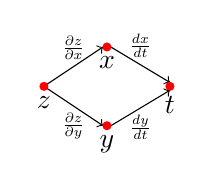
\begin{tikzpicture}
        \draw [->] (0,0) -- (0.75,0.5) node [midway, above, scale = 0.7] {$\frac{\partial z}{\partial x}$};
        \draw [->] (0,0) -- (0.75,-0.5) node [midway, below, scale = 0.7] {$\frac{\partial z}{\partial y}$};
        \draw [->] (0.85,0.5) -- (1.6,0.05) node [midway, above, scale = 0.7] {$\frac{dx}{dt}$};
        \draw [->] (0.85,-0.5) -- (1.6,-0.05) node [midway, below, scale = 0.7] {$\frac{dy}{dt}$};
        \draw [fill, red] (0,0) circle [radius=0.05];
        \draw [fill, red] (0.8,0.5) circle [radius=0.05];
        \draw [fill, red] (0.8,-0.5) circle [radius=0.05];
        \draw [fill, red] (1.6,0) circle [radius=0.05];
        \node [below] at (0,0) {$z$};
        \node [below] at (0.8,0.5) {$x$};
        \node [below] at (0.8,-0.5) {$y$};
        \node [below] at (1.6,0) {$t$};
      \end{tikzpicture}
      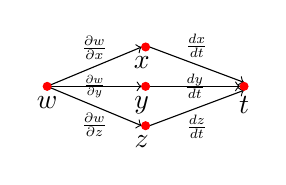
\begin{tikzpicture}
        \draw [->] (0,0) -- (1.2,0.5) node [midway, above, scale = 0.7] {$\frac{\partial w}{\partial x}$};
        \draw [->] (0,0) -- (1.2,-0.5) node [midway, below, scale = 0.7] {$\frac{\partial w}{\partial z}$};
        \draw [->] (0,0) -- (1.2,0) node [midway, scale = 0.6] {$\frac{\partial w}{\partial y}$};
        \draw [->] (1.3,0.5) -- (2.5,0.05) node [midway, above, scale = 0.7] {$\frac{dx}{dt}$};
        \draw [->] (1.3,-0.5) -- (2.5,-0.05) node [midway, below, scale = 0.7] {$\frac{dz}{dt}$};
        \draw [->] (1.3,0) -- (2.45,0) node [midway, scale = 0.7] {$\frac{dy}{dt}$};
        \draw [fill, red] (0,0) circle [radius=0.05];
        \draw [fill, red] (1.25,0.5) circle [radius=0.05];
        \draw [fill, red] (1.25,-0.5) circle [radius=0.05];
        \draw [fill, red] (1.25,0) circle [radius=0.05];
        \draw [fill, red] (2.5,0) circle [radius=0.05];
        \node [below] at (0,0) {$w$};
        \node [below] at (1.2,0.5) {$x$};
        \node [below] at (1.2,-0.5) {$z$};
        \node [below] at (1.2,0) {$y$};
        \node [below] at (2.5,0) {$t$};
      \end{tikzpicture}
    }
  \end{wrapfigure}

  $z = f(x,y), \\x=x(t), y=y(t)$

  $w = f(x,y,z), \\x=x(t), \\y=y(t), z=z(t)$

  \subsection*{Directional Derivative}
  $f_x(a,b)$ is rate of change of $f$ along direction of x-axis

  Directional derivative of $f$ at $(a,b)$ in direction of unit vector $u = u_1\mathbf{i} + u_2\mathbf{j}$ is $D_uf(a,b)=f_x(a,b)u_1 + f_y(a,b)u_2$

  or $D_uf(a,b,c)=f_x(a,b,c)u_1 + f_y(a,b,c)u_2 + f_z(a,b,c)u_3$

  $df = D_uf(a,b)\cdot dt$ (normal $\cdot$ multiplication) measures change in $f$ ($df$) when we move a small distance $dt$, and $u$ is the unit directional vector of the change and $(a,b)$ is the original pt

  \subsection*{Gradient Vector}
  Denoted by $\nabla f = f_x\mathbf{i} + f_y\mathbf{j}$ where

  $\nabla f(a,b) \cdot u = D_uf(a,b) = \lVert\nabla f(a,b)\rVert\cos\theta$

  $D_uf(a,b) >0$ and max when $\cos \theta = 1 \iff \theta = 0^{\circ}$

  $D_uf(a,b) <0$ and min when $\cos \theta = -1 \iff \theta = 180^{\circ}$

  \subsection*{Max and Min Values}
  \textbf{Critical Points - First Derivative Test}

  $f$ has a local max or min at $(a,b) \land f_x$ exists $\land f_y$ exists $\rightarrow$ $f_x=0 \land f_y=0$ (But not the converse)

  \textbf{Second Derivative Test}

  Disriminant = $f_{xx}(a,b)f_{yy}(a,b) - f_{xy}(a,b)^2$
  \begin{enumerate}
    \item $D>0 \land f_{xx}(a,b)>0 \rightarrow f$ has	a local min at $(a,b)$
    \item $D>0 \land f_{xx}(a,b)<0 \rightarrow f$ has a local max at $(a,b)$
    \item $D<0 \rightarrow f$ has a saddle-point at $(a,b)$
    \item $D = 0 \rightarrow$ no conclusion
  \end{enumerate}


  \section{Ordinary Differential Equation (ODE)}
  \textbf{No Crossing Principle}: solution curves do not cross each other
  \subsection*{First order ODE}
  There is only 1 soln for initial value problem with 1st order ODE. Intersection point of 2 curves is the initial pt.
  \begin{enumerate}
    \item $\frac{dy}{dx} = \frac{M(x)}{N(y)} \iff \int M(x)dx = \int N(y)dy$
    \item $y' = f(\frac{y}{x}) \Leftrightarrow $ Let $v=\frac{y}{x}, f(v) = y'\Leftrightarrow \frac{dv}{f(v)-v}=\frac{dx}{x}$
    \item $y'=\frac{ax+by+c}{a_1x+b_1y+c_1} \Leftrightarrow$ Let $u = ax+by$
    \item $\frac{dy}{dx}+p(x)y = Q(x) \Leftrightarrow ye^{\int p(x)dx}=\int Q(x)e^{\int p(x)dx}dx$
    \item \textbf{Bernoulli eqn} $y' + p(x)y = q(x)y^n \Leftrightarrow $\\
          Let $z=y^{1-n} \Leftrightarrow z' + (1-n)p(x)z = (1-n)q(x)$
  \end{enumerate}
  \subsection*{Scenarios}
  Radioactive decay: $\frac{dx}{dt} = kx$, $x(t)=x(0)e^{-\frac{\ln 2}{\tau}t}$

  Uranium-Thorium: ${\frac{T}{U}=\frac{k_U}{k_T-k_U}(1-e^{-(k_T-k_U)t}) k_N = \frac{\ln 2}{\tau_N}}$

  Cooling/Heating: $\int\frac{dT}{T-T_0}=\int kdt$, $T(t) - T_0 = (T(0) - T_0)e^{kt}$

  Retarded fall: $m\frac{dv}{dt} = mg-bv^2,$\\
  $v = k\frac{1 + ce^{-pt}}{1-ce^{-pt}}, k^2 = \frac{mg}{b},c = \frac{v(0)-k}{v(0)+k}, p=\frac{2kb}{m}$
  \subsection*{Hyperbolic Functions}
  ${\cosh x=\frac{e^x + e^{-x}}{2}, \sinh x = \frac{e^x + e^{-x}}{2}, \tanh x=\frac{\sinh x}{\cosh x}=\frac{1-e^{-2x}}{1+e^{-2x}}}$

  \subsection*{Second order linear ODE}
  Form: $\frac{d^2y}{dx^2}+p(x)\frac{dy}{dx}+q(x)y=F(x)$

  homogeneous $\Leftrightarrow F(x)=0$, else non-homogeneous



  \subsection*{Homogeneous 2nd order linear ODE}
  \textbf{Linearly dependent} ${\Leftrightarrow \forall x \exists c\text{ s.t. }u(x)=cv(x)}$

  $y_1, y_2$ are lin. indep. solns $\Rightarrow$ a general soln is $y=c_1y_1+c_2y_2$

  $y_1,y_2$ are NOT lin. indep. solns $\Rightarrow y=c_1y_1+c_2y_2$ is a soln but not a general soln

  $\frac{d^2y}{dx^2}+A\frac{dy}{dx}+By=0$ has the trivial soln $y=0$ and non-trivial soln: Let $y=e^{\lambda x}$, solve $\lambda^2+A\lambda+B=0$, general soln is: (PS: Reverse is $A=-(\lambda_1 + \lambda_2), B=\lambda_1 \lambda_2$)
  \begin{enumerate}
    \item 2 real roots: ${y=c_1e^{\lambda_1x}+c_2e^{\lambda_2x}}$
    \item 1 real root: $y=c_1e^{\lambda_1x}+c_2xe^{\lambda_1x}$
    \item 2 complex roots ($a+ib$): ${y=e^{ax}(c_1\cos bx + c_2\sin bx)}$
  \end{enumerate}
  \section{Mathematical Modelling (B = birth rate, D = death rate)}
  \subsection*{Malthusian Population Growth }
  $N(t) = N(0)e^{kt}$ where $k=B-D$. Conditions:
  \begin{enumerate}
    \item $k>0$ ($B>D$): popn explosion ($e^{kt}\to\infty, N(t)\to\infty$ as $t\to\infty$)
    \item $k=0$ ($B=D$): stable ($N(t)=N(0)$ for all $t$)
    \item $k<0$ ($B<D$): extinction ($e^{kt}\to0, N(t)\to0$ as $t\to\infty$)
  \end{enumerate}
  \subsection*{Logistic Growth Model}
  \begin{tikzpicture}
    \begin{axis}[
        xmin=-6,xmax=6,xticklabels={,,},
        axis x line=bottom,
        ytick={0,.5,1},yticklabels={,,},ymax=1,
        axis y line=left,
        height=3.5cm
      ]
      \addplot[blue,mark=none,samples=100,domain=-6:6](x,{1/(1+exp(-x))});
      \addplot[blue,mark=none,samples=100,domain=-6:6](x,{1/(1+exp(-x))});
    \end{axis}
  \end{tikzpicture}\\
  Eqn: $\frac{dN}{dt}=(B-D)N, N(0) = \hat{N}, N_\infty=\frac{B}{s}$\\
  $\frac{dN}{dt}=(B-D)N = (B-sN)N = BN-sN^2$ where $s$ is a small number compared to $B$.\\
  $\frac{dN}{dt}=0$ when $N \approx \frac{B}{s}$ (population stops growing)\\
  This constant $\frac{B}{s}$ is called carrying capacity, sustainable population, or logistic equilibrium population. Or that the population stabilises at $\frac{B}{s}$\\
  $N(t) = \frac{B}{s+\left(\frac{B}{N_0}-s\right)e^{-Bt}}= \frac{N_\infty}{1 + (\frac{N_\infty}{N_0}-1)e^{-Bt}}$\\
  $\lim\limits_{t\to\infty} N(t) = \frac{B}{s}$\\
  \textbf{Case 1: $B - sN(t) > 0\ \forall t$ (Popn < sustainable popn)}\\
  Logistic curve increasing\\
  \textbf{Case 2: $B -sN(t) < 0$ at all $t$ (Popn > sustainable popn)}\\
  Logistic curve decreasing\\
  \textbf{Case 3: $B -sN(t) = 0$ at all $t$ (At sustainable popn)}\\
  Population constant at $N(0)$\\
  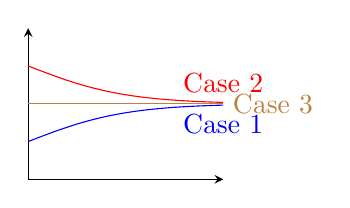
\begin{tikzpicture}
    \begin{axis}[
        xmajorticks=false,
        xmin=0,xmax=4,
        axis x line=bottom,
        ymajorticks=false,
        ymin=0,ymax=2,
        axis y line=left,
        height=3.5cm,
        clip=false
      ]
      \addplot[blue,mark=none,samples=100,domain=0:4](x,{1/(1+exp(-x))}) node[below,pos=1] {Case 1};
      \addplot[red,mark=none,samples=100,domain=0:4](x,{2-1/(1+exp(-x))})node[above,pos=1] {Case 2};
      \addplot[brown,mark=none,samples=100,domain=0:4](x,{1})node[right,pos=1] {Case 3};
    \end{axis}
  \end{tikzpicture}\\
  \subsection*{Harvesting}
  $\frac{dN}{dt}=BN-sN^2-E$ where $E$ is fish caught per year.\\
  \textbf{DO NOT ATTEMPT TO SOLVE THE ODE.} They will just ask to draw graph.\\
  Method:
  \begin{enumerate}
    \item Let $F(N) = \frac{dN}{dt} = -sN^2 + BN -E$
    \item Discriminant = $B^2 - 4(-s)(-E) = B^2 - 4sE$
    \item Cases:
          \begin{enumerate}
            \item $D<0$: No equiblirium soln (Popn is decreasing to extinction)\\
                  Note: $-s<0$, shape is $\cap$, $F(N)\neq0$\\
                  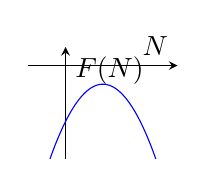
\begin{tikzpicture}
                    \begin{axis}[
                        xmajorticks=false,
                        xmin=-2,xmax=6,
                        xlabel={$N$},
                        axis x line=center,
                        ymajorticks=false,
                        ymin=-10,ymax=2,
                        ylabel={$F(N)$},
                        axis y line=center,
                        height=3cm,
                      ]
                      \addplot[blue,mark=none,samples=100,domain=-2:6](x,{-2-(x-2)^2});
                    \end{axis}
                  \end{tikzpicture}
                  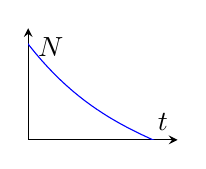
\begin{tikzpicture}
                    \begin{axis}[
                        xmajorticks=false,
                        xmin=0,xmax=2,
                        xlabel={$t$},
                        axis x line=center,
                        ymajorticks=false,
                        ymin=0,ymax=7,
                        ylabel={$N$},
                        axis y line=center,
                        height=3cm,
                      ]
                      \addplot[blue,mark=none,samples=100,domain=-2:6](x,{6-1/3*x^3 + 2*x^2 - 6*x});
                    \end{axis}
                  \end{tikzpicture}
            \item $D>0$: 2 equilibrium solns\\
                  Solve $F(N)$ for $\beta_1, \beta_2$ where $\beta_1<\beta_2<\frac{B}{s}$\\
                  There are 3 possible cases:\\
                  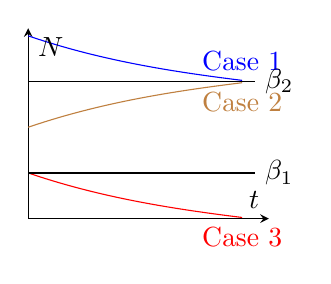
\begin{tikzpicture}
                    \begin{axis}[
                        xmajorticks=false,
                        xmin=0,xmax=1.8,
                        xlabel={$t$},
                        axis x line=center,
                        ymajorticks=false,
                        ymin=0,ymax=25,
                        ylabel={$N$},
                        axis y line=center,
                        height=4cm,
                        clip=false
                      ]
                      \addplot[blue,mark=none,samples=100,domain=0:1.6](x,{24-1/3*x^3 + 2*x^2 - 6*x}) node[above,pos=1] {Case 1};
                      \addplot[brown,mark=none,samples=100,domain=0:1.6](x,{12-(-1/3*x^3 + 2*x^2 - 6*x)}) node[below,pos=1] {Case 2};
                      \addplot[red,mark=none,samples=100,domain=0:1.6](x,{6-1/3*x^3 + 2*x^2 - 6*x}) node[below,pos=1] {Case 3};
                      \addplot[black,mark=none,samples=100,domain=0:1.7](x, {18}) node [right, pos=1] {$\beta_2$};
                      \addplot[black,mark=none,samples=100,domain=0:1.7](x, {6}) node [right, pos=1] {$\beta_1$};
                    \end{axis}
                  \end{tikzpicture}\\
                  $\frac{B}{s}=\beta_1+\beta_2, \frac{E}{s}=\beta_1\beta_2$\\
                  $\beta_2$ is stable ($N(0)$ slightly diff from $\beta_2$, popn will still tend to $\beta_2$). $\beta_1$ is not stable ($N(0)$ slightly diff from $\beta_1$ will not tend to $\beta_1$)
            \item $D=0$: 1 equilibrium solns\\
                  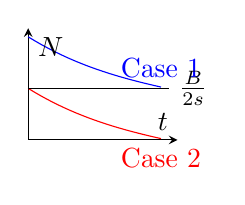
\begin{tikzpicture}
                    \begin{axis}[
                        xmajorticks=false,
                        xmin=0,xmax=1.8,
                        xlabel={$t$},
                        axis x line=center,
                        ymajorticks=false,
                        ymin=0,ymax=13,
                        ylabel={$N$},
                        axis y line=center,
                        height=3cm,
                        clip=false
                      ]
                      \addplot[blue,mark=none,samples=100,domain=0:1.6](x,{12-1/3*x^3 + 2*x^2 - 6*x}) node[above,pos=1] {Case 1};
                      \addplot[red,mark=none,samples=100,domain=0:1.6](x,{6-1/3*x^3 + 2*x^2 - 6*x}) node[below,pos=1] {Case 2};
                      \addplot[black,mark=none,samples=100,domain=0:1.7](x, {6}) node [right, pos=1] {$\frac{B}{2s}$};
                    \end{axis}
                  \end{tikzpicture}\\
                  Suppose $N(0)>\frac{B}{2s}$ then max. harvesting w/o extinction $E=\frac{B^2}{4s}$
          \end{enumerate}
  \end{enumerate}
  PS: more precise curves, follow the original logistic growth model graph (S-shaped) increasing: gentle-steep-gentle, decreasing: steep-gentle-steep
  \subsection*{Additional Notes}
  \begin{descitemize}
    \item If the question is in powers above 2, e.g. $\frac{dN}{dt}=aN^4+bN^3+cN^2+dN+e$, the same rule about the graph still applies: the stable populations are the solutions to $aN^4+bN^3+cN^2+dN+e=0$
    \item If there is no harvesting, then $N=0$ is also a solution.
  \end{descitemize}


\end{multicols*}
\end{document}
